\chapter{DAGDA extension}
\textsc{DAGDA} (\textbf{D}ata \textbf{A}rrangement for \textbf{G}rid and
\textbf{D}istributed \textbf{A}pplications) is a new data manager for DIET.
DAGDA offers  to the DIET application developers a simple and efficient way 
to manage the data. It was not designed to replace the JuxMem extension
but to be possibly coupled with it. In a future work, DAGDA will be
divided in two parts: The DAGDA data manager and the DAGDA data interface.
The data interface will make interactions between DAGDA, JuxMem, FTP
etc. and other data transfer/management protocols. In this chapter, we will
present the current version of DAGDA which is an alternative data manager
for DIET with several advanced data management features.
\section{Overview}
DAGDA allows data explicit or
implicit replications and advanced data management on the grid. It was
designed to be backward compatible with previously developed
applications for DIET which benefit transparently of the data
replications. Moreover, DAGDA limits the data size loaded in memory to
a user-fixed value and avoids CORBA errors when transmitting too large
data regarding to the ORB configuration.

DAGDA offers a new way to manage the data on DIET. The API allows the
application developer to replicate, move, add or delete a data to be
reused later or by another application. Each component of DIET can
interact with DAGDA and the data manipulation can be done from a
client application, a server or an agent through a plug-in
scheduler.

A DAGDA component is associated to each element in a DIET platform
(client, Master Agent, Local Agent, SeD). These components are connected
following the DIET deployment topology. Figure \ref{fig:DAGDAarch} shows how
the DAGDA and DIET classical components are connected. In contrary of a DIET
architecture, each DAGDA component has the same role. It can store, transfer
or move a data. The client's DAGDA component is isolated of the architecture and
communicates only with the chosen SeDs DAGDA components when necessary. When
searching for a data, DAGDA uses its hierarchical topology to contact the
data managers. Among the data managers having one replicate of the data,
DAGDA chooses the \textit{"best"} source to transfer it. To make this choice
DAGDA uses some statistics collected from previous data transfers between
the nodes. By not using dynamic information, it is unsure that DAGDA really
chose the "best" nodes for the transfers. In a future version, we will
introduce some facilities to estimate the time needed to transfer a data and
to improve the choice of a data stored on the grid. To do the data transfers,
DAGDA uses the pull model: It is the destination node that ask for the data
transfer.
\begin{figure}[h]
\centerline{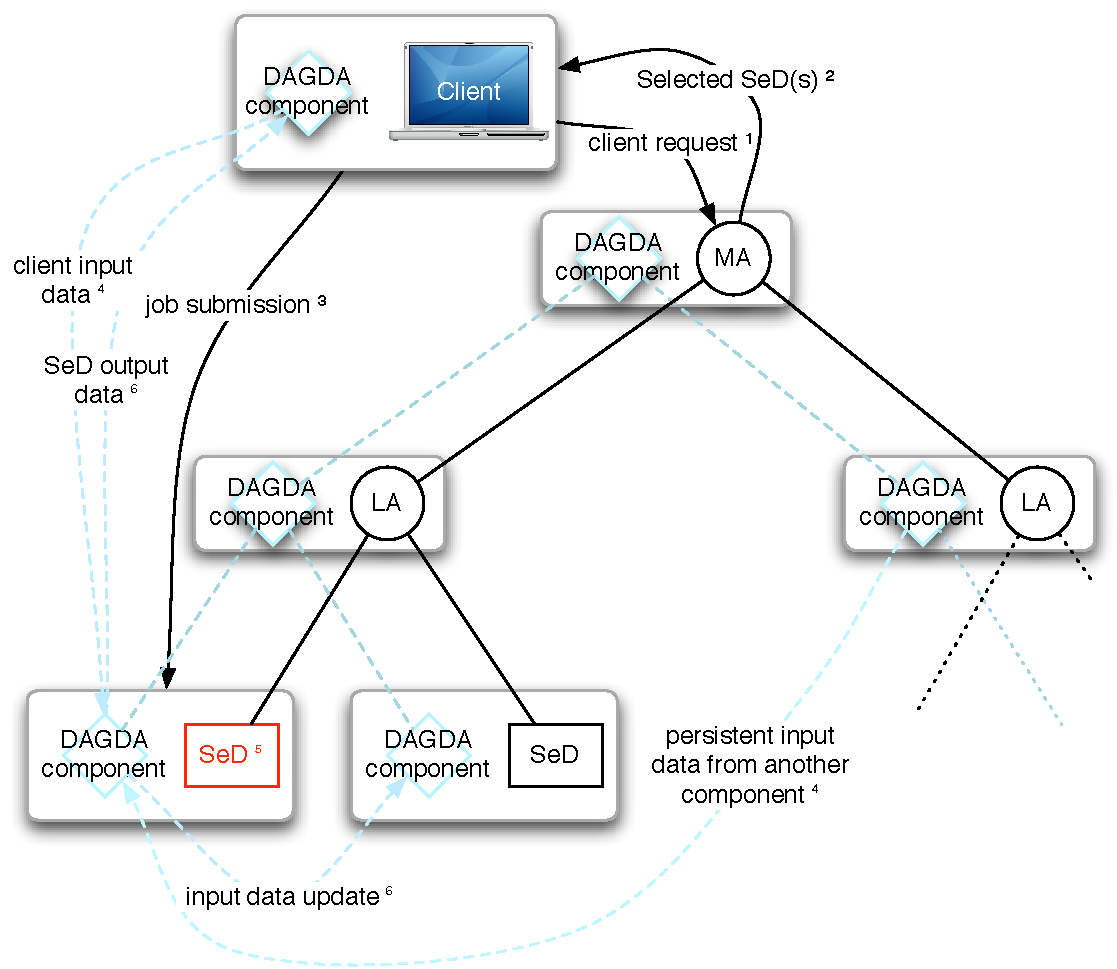
\includegraphics[width=0.7\linewidth]{fig/dagdaArch}}
\caption{DAGDA architecture in DIET.\label{fig:DAGDAarch}}
\end{figure}

Figure \ref{fig:DAGDAarch} presents how DAGDA manages the data when a client
submit a job. In this example, the client wants to use some data stored on the
grid and some personal data. He wants to obtain some results and to store
some others on the grid. Some of these output data are already stored on the
platform and they should be updated after the job execution.
\begin{enumerate}
  \item The client sends a request to the Master Agent.
  \item The Master agent returns one or more SeD references.
  \item The client sends its request to the chosen node. The parameters data
    are identified by a unique ID and the problem profile contains a reference
    to the client's data manager.
  \item Receiving the request the SeD asks the client to transfer the data of
    the user and it asks to the DAGDA architecture to obtain the persistent
    data already stored on the platform.
  \item The SeD executes the job. After the execution, the SeD stores the
    output data and it informs the client that the data are ready to be
    downloaded. It also asks to the architecture to update the modified output
    data.
  \item The client upload its results and the data are updated on the nodes.
\end{enumerate}

%Using DAGDA, each data stored on the platform can be replicated as many
%time as there is free space on the platform. To avoid DIET to take up all
%the storage ressources (disk or memory) of the nodes, DAGDA allows to fix
%a limit to the data size that can be stored for each DAGDA component. When
%a job needs a data, it asks DAGDA for it using its unique ID and gets it
%from the "best source". DAGDA uses some statistic informations to determine
%which node should be used for the transfers, but could be easily extended to
%use some dynamic metrology parameters. DAGDA also offers a way to manage
%automatically the data by choosing a \textit{cache replacement algorithm}
%for each node. The user can choose a persistence mode for each replica:
%\begin{itemize}
%  \item[-] Persistent: The data is kept as long as possible on the node
%    but can be deleted when the node needs some storage resources.
%  \item[-] Sticky: The data will stay on the node until a user chooses
%    to delete it explicitly.
%\end{itemize}
%Then, the three cache replacement algorithms implemented in DAGDA work as
%follows:
%\begin{itemize}
%  \item \emph{Least Recently Used} (LRU): The least recently used persistent
%    data of sufficient size is deleted.
%  \item \emph{Least Frequently Used} (LFU): The least frequently used
%    persistent data of sufficient size is deleted.
%  \item \emph{First In First Out} (FIFO): Among the persistent data of
%    sufficient size, the \textit{oldest} is deleted.
%\end{itemize}
%None of the above algorithms controls if another replica of the data
%exists on the platform before to delete it. The only way to ensure
%at least one replica of a data leaves on the platform is to declare
%one of them as \emph{sticky} data.

%Extending the DIET API, DAGDA allows to explicitly manage the data in the
%platform by communicating directly with the DAGDA hierarchy. However, DAGDA
%does not deal with the replicas consistency and the data availability. The
%user is responsible of what he does with the data. Even if DAGDA offers
%a way to update a persistent data, if a job or a user modifies the data
%while the updating process is executing, some side effects can appear.

\newcommand{\tabCell}[2]{%
  \begin{minipage}{#1}
    \vspace*{1mm}
    \scriptsize #2
    \vspace*{1mm}
  \end{minipage}
}
\section{The DAGDA configuration options}
DAGDA introduces new configuration options that can be defined for all the
DAGDA components. None of these options are mandatory to use DAGDA. Figure
\ref{fig:DAGDAoptions} presents all the DAGDA available options, their meaning
and default values.
\begin{figure}[h]
\begin{tabular}{|l|l|l|c|c|c|}
\hline
%& & & & & \\
\tabCell{2.9cm}{\vspace*{0.5cm}\centering\textbf{Option}} &
\tabCell{5cm}{\vspace*{0.5cm}\centering\textbf{Description}} &
\tabCell{4cm}{\vspace*{0.5cm}\centering\textbf{Default value}} &
\rotatebox{270}{\centering\bf Client} & \rotatebox{270}{\centering\bf Agent } &
\rotatebox{270}{\centering\bf SeD} \\
%& & & & &\\
\hline
%& & & & &\\
storageDirectory &
\tabCell{5cm}{The directory on which DAGDA will store the data files} &
\tabCell{4cm}{The \textit{/tmp} directory.} &
\ding{52} & \ding{52} & \ding{52} \\
%& & & & &\\
\hline
maxMsgSize &
\tabCell{5cm}{The maximum size of a CORBA message sent by DAGDA.} &
\tabCell{4cm}{The omniORB \textit{giopMaxMsgSize} size.} &
\ding{52} & \ding{52} & \ding{52} \\
%& & & & &\\
\hline
maxDiskSpace &
\tabCell{5cm}{The maximum disk space used by DAGDA to store the data. If set
to 0, DAGDA will not take care of the disk usage.} &
\tabCell{4cm}{The available disk space on the disk partition chosen by the
  \textit{storageDirectory} option.} &
\ding{52} & \ding{52} & \ding{52} \\
\hline
maxMemSpace &
\tabCell{5cm}{The maximum memory space used by DAGDA to store the data. If set
to 0, DAGDA will not take care of the memory usage.} &
\tabCell{4cm}{No maximum memory usage is set. Same effect than to choose 0.} &
\ding{52} & \ding{52} & \ding{52} \\
\hline
cacheAlgorithm &
\tabCell{5cm}{The cache replacement algorithm used when DAGDA needs more space
to store a data. Possible values are: \textit{LRU, LFU, FIFO}} &
\tabCell{4cm}{No cache replacement algorithm. DAGDA never replace a data by
another one.} &
\ding{52} & \ding{52} & \ding{52} \\
\hline
shareFiles &
\tabCell{5cm}{The DAGDA component shares its file data with all its children
(when the path is accessible by them, for example, if the storage directory is
on a NFS partition). Value can be 0 or 1.} &
\tabCell{4cm}{No file sharing - 0} &
\ding{56} & \ding{52} & \ding{56} \\
\hline
dataBackupFile &
\tabCell{5cm}{The path to the file that will be used when DAGDA save all its
stored data/data path when asked by the user (Checkpointing).} &
\tabCell{4cm}{No checkpointing is possible.} &
\ding{56} & \ding{52} & \ding{52} \\
\hline
restoreOnStart &
\tabCell{5cm}{DAGDA will load the \textit{dataBackupFile} file at start and
restore all the data recorded at the last checkpointing event. Possible values
are 0 or 1.} &
\tabCell{4cm}{No file loading on start - 0} &
\ding{56} & \ding{52} & \ding{52} \\
\hline
\end{tabular}
\caption{DAGDA configuration options}
\label{fig:DAGDAoptions}
\end{figure}

\section{Cache replacement algorithm}
When a data is replicated on a site, it is possible that not enough
disk/memory space is available. In that case, DAGDA allows to choose
a strategy to delete a persistent data. Only a simple persistent data
can be deleted, the sticky ones are never deleted by the chosen
algorithm. DAGDA offers three algorithm to manage the cache replacement:
\begin{itemize}
  \item LRU: The least recently used persistent data of sufficient size is
    deleted.
  \item LFU: The least frequently used persistent data of sufficient size
    is deleted.
  \item FIFO:  Among the persistent data of sufficient size, the
    \textit{oldest} is deleted.
\end{itemize}

\section{The DAGDA API}
By compiling DIET with the DAGDA extension activated, the
\textit{DIET\_Dagda.h} file is installed on the DIET include directory.
This file contains some data management functions and macros.
\subsection{Note on the memory management}
On the SeD side, DAGDA and the SeD share the
same data pointers, that means that if the pointer is a local variable
reference, when DAGDA will use the data, it will read an unallocated variable.
The users should allways allocate the data with a \textit{"malloc"/"calloc"} or
\textit{"new"} call on the SeD and agent sides. Because DAGDA takes the control
of the data pointer, there is no risk of memory leak even if the service
allocate a new pointer at each call. The data lifetime is managed by DAGDA
and the data will be freed according to its persistence mode.\\[4mm]
\begin{minipage}{2cm}
  \centering
  \textbf{{\Huge \Biohazard}}
\end{minipage}
\begin{minipage}{\textwidth - 2cm}
\textbf{On the SeD and agent sides, DAGDA takes the control of the data
pointers. To free a data may cause major bugs which could be very hard to
find. The users could only free a DIET data on the client side after the end of
a transfer.}
\end{minipage}
\subsection{Synchronous data transfers}
All of the following functions returns at the end of the transfer or
if an error occured. They all returns an integer value: 0 if the operation
succeed, another value if it failed.
\subsubsection{DAGDA \textit{put} data macros/functions.}
\label{sec:syncPutFunctions}
The following functions put a data on the DAGDA hierarchy to be used later.
The last parameter is allways a pointer to a C-string which will be
initialized with a pointer to the ID string of the data. This string is
allocated by DAGDA and can be freed when the user does not need it anymore.
The first parameter is allways a pointer to the data: For a scalar value
a pointer on the data, for a vector, matrix or string, a pointer on the
first element of the data. The \textit{"value"} argument for a file is
a C-string containing the path of this file. The persistence mode for
a data managed by DAGDA should allways be DIET\_PERSISTENT or DIET\_STICKY.
The VOLATILE and *\_RETURN modes do not make sense in this data management
context.

% \begin{itemize}
%   \item Synchronous: The called function returns when the transfer is ended.
%   \item Asynchronous with control: The called function returns immediately.
%     The user can wait the end of the transfer by calling to a DAGDA wait
%     function.
%   \item Asynchronous without control: The called function returns immediately.
%     The user cannot wait the end of the transfer. These functions should only
%     be used on the SeD or Agent sides.
% \end{itemize}
% \subsubsection{Synchronous data transfers.}
\begin{itemize}
  \item[-] \verb#dagda_put_scalar(void* value, diet_base_type_t base_type,#\\
           \verb#                 diet_persistence_mode_t mode, char** ID)#:\\
           This macro adds to the platform, the scalar data of type
           \textit{"base\_type"} pointed by \textit{"value"} with the
           persistence mode \textit{"mode"} (DIET\_PERSISTENT or DIET\_STICKY)
           and initializes \textit{"*ID"} with the ID of the data.
  \item[-] \verb#dagda_put_vector(void* value, diet_base_type_t base_type,#\\
           \verb#                 diet_persistent_mode_t mode, size_t size, char** ID)#:\\
           This macro adds to the platform, the vector of \textit{"size"}
           \textit{"base\_type"} elements pointed by \textit{"value"} with the
           persistence mode \textit{"mode"} and stores the data ID in
           \textit{"ID"}.
  \item[-] \verb#dagda_put_matrix(void* value, diet_base_type_t base_type,#\\
         \verb#                 diet_persistence_mode_t mode, size_t nb_rows,#\\
         \verb#                 size_t nb_cols, diet_matrix_order_t order, char** ID)#:\\
           This macro adds to the platform the \textit{"base\_type"} matrix of
           dimension \textit{"nb\_rows"} $\times$ \textit{"nb\_cols"} stored in
           \textit{"order"} order. The data ID is stored on \textit{"ID"}.
  \item[-] \verb#dagda_put_string(char* value, diet_persistence_mode_t mode, char** ID)#:\\
           This macro adds to the platform the string pointed by
           \textit{"value"} with the persistence mode \textit{"mode"} and
           stores the data ID into \textit{"ID"}.
  \item[-] \verb#dagda_put_file(char* path, diet_persistence_mode_t mode, char**ID)#:\\
           This macro adds the file of path \textit{"path"} with the persistence
           mode \textit{"mode"} to the platform and stores the data ID into
           \textit{"ID"}
 \end{itemize}

\subsubsection{DAGDA \textit{get} data macros/functions}
\label{sec:syncGetFunctions}
The following API functions are defined to obtain a data from DAGDA using
its ID:
\begin{itemize}
  \item[-] \verb#dagda_get_scalar(char* ID, void** value,#\\
           \verb#                 diet_base_type_t* base_type)#:\\
    The scalar value using the ID \textit{"ID"} is obtained from DAGDA and the
    \textit{"value"} argument is initialized with a pointer to the data.
    The \textit{"base\_type"} pointer content is set to the data base type.
    This last parameter is optionnal and can be set to NULL if the user does not
    want to get the \textit{"base\_type"} value.
  \item[-] \verb#dagda_get_vector(char* ID, void** value,#\\
           \verb#                 diet_base_type_t* base_type, size_t* size)#:\\
    The vector using the ID \textit{"ID"} is obtained from DAGDA. The
    \textit{"value"} argument is initialized with a pointer to the first
    vector element. The \textit{"base\_type"} content are initialized with
    the base type and size of the vector. These two parameters can be set to
    NULL if the user does not take care about it.
  \item[-] \verb#dagda_get_matrix(char* ID, void** value,#\\
           \verb#                 diet_base_type_t* base_type, size_t* nb_r,#\\
           \verb#                 size_t* nb_c, diet_matrix_order_t* order)#:\\
    The matrix using the ID \textit{"ID"} is obtained from DAGDA. The
    \textit{"value"} argument is initialized with a pointer to the first
    matrix element. The \textit{"base\_type"}, \textit{"nb\_r"},
    \textit{"nb\_c"} and \textit{"order"} arguments contents are repectively set
    to the base type of the matrix, the number of rows, the number of columns
    and the matrix order. All of these parameters can be set to NULL if the
    user does not take care about it.
  \item[-] \verb#dagda_get_string(char* ID, char** value)#:\\
    The string of ID \textit{"ID"} is obtained from DAGDA and the
    \textit{value} content is set to a pointer on the first string character.
  \item[-] \verb#dagda_get_file(char* ID, char** path)#:\\
    The file of ID \textit{"ID"} is obtained from DAGDA and the
    \textit{"path"} content is set to a pointer on the first path string
    character.
\end{itemize}

\subsection{Asynchronous data transfers.}
With DAGDA, there is two way to manage the asynchronous data transfers,
depending of the data usage:
\begin{itemize}
  \item With end-of-transfer control: DAGDA maintains a reference to the
    transfer thread. It only release this reference after a call to the
    corresponding waiting function. The client developer should allways use
    these functions, that's why a data ID is only returned by the
    \textit{"dagda\_wait\_*"} and \textit{"dagda\_wait\_data\_ID"} functions.
  \item Without end-of-transfer control: The data is loaded from/to the
    DAGDA hierarchy without the possibility to wait for the end of the transfer.
    These functions should only be called from an agent plugin scheduler, a
    SeD plugin scheduler or a SeD if the data transfer without usage of the
    data is one of the objectives of the called service. The data adding
    functions without control should be used very carefully because there is
    no way to be sure the data transfer is achieved or even started.    
\end{itemize}
With asynchronous transfers, the user should take care of the data lifetime
because DAGDA does not duplicate the data pointed by the passed pointer.
For example, if the program uses a local variable reference to add a data
to the DAGDA hierarchy and go out of the variable scope, a crash could
occured because the data pointer could be freed by the system before DAGDA has
finished to read it.
\subsubsection{DAGDA asynchronous \textit{put} macros/functions}
The arguments to these functions are the same than for the synchronous ones.
See Section \ref{sec:syncPutFunctions} for more details. All of these functions
return a reference to the data transfer which is an unsigned int. This value
will be passed to the \textit{"dagda\_wait\_data\_ID"} function.
\begin{itemize}
\item[-] \verb#dagda_put_scalar_async(void* value, diet_base_type_t base_type,#\\
         \verb#                       diet_persistence_mode_t mode)#
\item[-] \verb#dagda_put_vector_async(void* value, diet_base_type_t base_type,#\\
         \verb#                       diet_persistence_mode_t mode, size_t size)#
\item[-] \verb#dagda_put_matrix_async(void* value, diet_base_type_t base_type,#\\
         \verb#                       diet_persistence_mode_t mode, size_t nb_rows,#\\
         \verb#                       size_t nb_cols, diet_matrix_order_t order)#
\item[-] \verb#dagda_put_string_async(char* value, diet_persistence_mode_t mode)#
\item[-] \verb#dagda_put_file_async(char* path, diet_persistence_mode_t mode)#
\end{itemize}
After calling to one of these functions, the user can obtain the data ID by
calling to the \textit{"dagda\_wait\_data\_ID"} function by using a transfer
reference.
\begin{itemize}
  \item[-] \verb#dagda_wait_data_ID(unsigned int transferRef, char** ID)#:\\
    The \textit{"transferRef"} argument is the value returned by a
    \textit{"dagda\_put\_*\_async"} function. The \textit{"ID"} content will
    be initialized to a pointer on the data ID.
\end{itemize}

\subsubsection{DAGDA asynchronous \textit{get} macros/functions}
The only argument needed for one of these functions is the data ID.
All of these functions return a reference to the data transfer which is an
unsigned int. This value will be passed to the corresponding
\textit{"dagda\_wait\_*"} functions described later.
\begin{itemize}
\item[-] \verb#dagda_get_scalar_async(char* ID)#
\item[-] \verb#dagda_get_vector_async(char* ID)#
\item[-] \verb#dagda_get_matrix_async(char* ID)#
\item[-] \verb#dagda_get_string_async(char* ID)#
\item[-] \verb#dagda_get_file_async(char* ID)#
\end{itemize}

After asking for an asynchronous transfer, the user has to wait for the end
of it by calling the corresponding \textit{"dagda\_wait\_*"} function.
The arguments to these functions are the same than for the synchronous
\textit{"dagda\_get\_*"} functions. See Section \ref{sec:syncGetFunctions}
for more details.

\begin{itemize}
\item[-] \verb#dagda_wait_scalar(unsigned int transferRef, void** value,#\\
         \verb#                  diet_base_type_t* base_type)#
\item[-] \verb#dagda_wait_vector(unsigned int transferRef, void** value,#\\
         \verb#                  diet_base_type_t* base_type, size_t* size)#
\item[-] \verb#dagda_wait_matrix(unsigned int transferRef, void** value,#\\
         \verb#                  diet_base_type_t* base_type, size_t* nb_r,#\\
         \verb#                  size_t* nb_c, diet_matrix_order_t* order)#
\item[-] \verb#dagda_wait_string(unsigned int transferRef, char** value)#
\item[-] \verb#dagda_wait_file(unsigned int transferRef, char** path)#
\end{itemize}

It is frequent that a plugin scheduler developer wants to make an asynchronous
data transfer to the local DIET node. In that case, to wait the end of the
transfers before to return can be a problem. But with the previously defined
functions, DAGDA maintains a reference to the transfer thread which will be
released after a call to the waiting function. To avoid DAGDA to keep
infinitely these references, the user should call the \textit{"dagda\_load\_*"}
functions instead of the \textit{"dagda\_get\_*\_async"} ones.

\begin{itemize}
\item[-] \verb#dagda_load_scalar(char* ID)#
\item[-] \verb#dagda_load_vector(char* ID)#
\item[-] \verb#dagda_load_matrix(char* ID)#
\item[-] \verb#dagda_load_string(char* ID)#
\item[-] \verb#dagda_load_file(char* ID)#
\end{itemize}

\subsection{Data checkpointing with DAGDA}
DAGDA allows the SeD administrator to choose a file where DAGDA will store
all the data that it manages. When a SeD has a configured valid path name to a
backup file (\textit{"dataBackupFile"} option in the configuration file),
a client can ask to the agents or SeDs DAGDA components to save the data.\\

The \verb#dagda_save_platform()# function, which can only be
called from a client, records all the data managed by the agents or SeDs DAGDA
components that allow it.\\
Then, the \textit{"restoreOnStart"} configuration file option asks to the
DAGDA component to restore the data stored on the \textit{"dataBackupFile"}
file when the component starts. This mechanism allows to stop the DIET
platform for a while and to restart it conserving the same data distribution.

\subsection{Create data ID aliases.}
For many applications using large sets of data shared by several users, to
use an automatically generated ID to retrieve a data is impossible or difficult.
DAGDA allows the user to define data aliases, using human readable and
expressive strings to retrieve a data ID. Two functions are defined to do it:
\begin{itemize}
\item[-] \verb#dagda_data_alias(const char* id, const char* alias)#:\\
  Tries to associate \textit{"alias"} to \textit{"id"}. If the alias is
  already defined, returns a non zero value. A data can have several aliases
  but an alias is allways associated to only one data.
\item[-] \verb#dagda_id_from_alias(const char* alias, char** id)#:\\
  This function tries to retrieve the data id associated to the alias.
\end{itemize}

\subsection{Data replication}
After a data has been added to the DAGDA hierarchy, the users can choose to
replicate it explicitely on one or several DIET nodes. With the current
DAGDA version, we allow to choose the nodes where the data will be replicated
by hostname or DAGDA component ID. In future developments, it will be
possible to select the nodes differently. To maintain backward compatibility,
the replication function uses a C-string to define the replication rule.
\begin{itemize}
\item[-] \verb#dagda_replicate_data(const char* id, const char* rule)#
\end{itemize}
The replication rule is defined as follows:\\
"$<$Pattern target$>$:$<$identification pattern$>$:$<$Capacity overflow
behavior$>$"\\
\begin{itemize}
\item The \textit{pattern target} can be "ID" or "host".
\item The \textit{identification pattern} can contain some \textit{wildcards}
  characters. (for example \textit{"*.lyon.grid5000.fr"} is a valid pattern.
\item The \textit{capacity overflow behavior} can be "replace" or "noreplace".
  "replace" means the cache replacement algorithm will be used if available on
  the target node (a data could be deleted from the node to leave space to
  store the new one). "noreplace" means that the data will be replicated on
  the node if and only if there is enough storage capacity on it.
\end{itemize}

For example, \textit{"host:capricorne-*.lyon.*:replace"} is a valid replication
rule.

\section{On correct usage of DAGDA}
Some things to keep in mind when using DAGDA as data manager for
DIET:
\begin{itemize}
\item All the data managed by DAGDA are entirely managed by DAGDA: The user
  must not free them. DAGDA avoids memory leaks, so the user does not
  have to worry about the memory management for the data managed by DAGDA.
\item When using more than one DAGDA component on a node, the user should
  define a different storage directory for each component. For example,
  the Master Agent and one SeD are launched on the same computer: the
  user can define the storage directory of the Master Agent as ``/tmp/MA''
  and the one for the SeD as ``/tmp/SeD1''. Do not forget to create the
  directories before to use DAGDA. This tip avoids many bugs which are
  really hard to find.
\item The DAGDA API can be used to transfer the parameters of a service,
  but it should not be used as this. If an application needs a data which
  is only on the client, the user should transmit it through the profile.
  The DAGDA API should be used to share, replicate or retrieve an existing
  data. Using the API allows the user to optimize their applications, not
  to proceed to a diet\_call even if it works fine. Indeed, the DAGDA
  client component is not linked to the DIET hierarchy, so using the API to
  add a data and then to use it as a profile parameter makes DAGDA to
  do additionnal and useless transfers.
\item DAGDA can be used without any configuration, but it is allways a
  good idea to define all the DAGDA parameters in the configuration files.
\end{itemize}

For any comment or bug report on DAGDA, please contact G. Le Mahec
at the following e-mail address: \url{gael.le.mahec@ens-lyon.fr}.

\section{Future works}
The next version of DAGDA will allow the users to develop their own cache
replacement algorithms and network capacity measurements methods.
DAGDA will be separated in two parts: A data management interface and a the
DAGDA data manager itself. DAGDA will implement the GridRPC data management API
extension.